\documentclass{standalone}
\usepackage{../../../../preamble_tikz}

\begin{document}

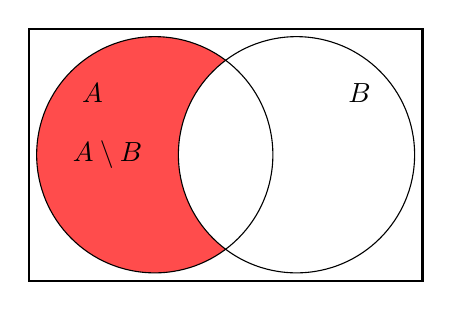
\begin{tikzpicture}
  \draw[thick] (-1.6,-1.6) rectangle (3.4,1.6);
  % Set A
  \node[circle,minimum size = 3cm,label={[label distance=-0.75cm]135:$A$},fill=red!70] (A) at (0,0) {}; %"minimum size" is the diameter. "label={135:$A$}" positions texts $A$ at 135 degrees of the circle. 

  % Set B
  \node[circle,minimum size = 3cm,label={[label distance=-0.75cm]45:$B$},fill=white] (B) at (1.8,0) {};
  %"minimum size" is the radius. "label={45:$B$}" positions texts $B$ at 45 degrees of the circle. 

  % Draw circle outline
  \draw (0,0) circle(1.5cm);
  \draw (1.8,0) circle(1.5cm);

  % Set intersection label
  \node at (-0.6,0) {$A\setminus B$};
\end{tikzpicture}
\end{document}